\documentclass[11pt,twoside,a4paper]{article}
\title{MCMC Convergence and Tessellation Budget Sensitivity
in the AddiVortes Model}
\author{Lewis Maltby, supervised by Prof.\ John Paul Gosling}
\usepackage{amsmath}
\usepackage[margin=0.8in]{geometry}
\usepackage[colorlinks=true, urlcolor=blue, linkcolor=black, citecolor=black]{hyperref}
\usepackage{graphicx}
\usepackage{subcaption}
\usepackage{booktabs}
\usepackage{adjustbox}
\usepackage{cite}
\bibliographystyle{unsrt}
\usepackage{float}
\usepackage{tcolorbox}
\usepackage{longtable}
\usepackage{array}
\usepackage{listings}
\usepackage{xcolor}
\usepackage{hyperref}
\usepackage{parskip}
\usepackage{csvsimple}
\usepackage[strings]{underscore}
\tcbuselibrary{listings}
\raggedbottom
\hypersetup{
    colorlinks=true,
    linkcolor=blue,
    urlcolor=blue,
    citecolor=blue
}

\lstdefinestyle{Rstyle}{
    language=R,
    basicstyle=\ttfamily\small,
    keywordstyle=\color{blue},
    commentstyle=\color{gray},
    stringstyle=\color{teal},
    numbers=left,
    numberstyle=\tiny\color{gray},
    breaklines=true,
    frame=single,
    backgroundcolor=\color{gray!5},
    showstringspaces=false
}
\begin{document}
\begin{titlepage}
    \centering
    
    {\scshape\LARGE Durham University \par}
    \vspace{1.5cm}
    
    {\huge\bfseries MCMC Convergence and Tessellation Budget Sensitivity
in the AddiVortes Model\par}
    \vspace{2cm}
    
    {\Large Lewis Maltby\par}
    \vspace{1cm}
    
    \vfill
    
    {\large Supervised by\par}
    {\Large Prof.\ John Paul Gosling\par}
	{\Large Dmitry Nikolaenko, RSE\par}    
    
    \vfill
    
    {\large \today\par}

\end{titlepage}
\setcounter{page}{1}
\section{Introduction}
The Additive Voronoi Tessellations (AddiVortes) model is a multivariate regression model that uses Voronoi tessellations to partition the covariate space in an additive ensemble model. Unlike other partition methods, such as decision trees, this has the benefit of allowing the boundaries of the partitions to be non-orthogonal and nonparallel to the covariate axes. The AddiVortes model uses a similar sum-of-tessellations approach and a Bayesian backfitting MCMC algorithm to the BART model. We use regularization priors to limit the strength of individual tessellations and accepts new models based on a likelihood.\cite{main-paper}
\\\\
Two lesser understood aspects of the AddiVortes model are MCMC convergence and budget sensitivity. We want to be able to better understand MCMC convergence behaviour as the dimensionality of the problem (the number of input covariates), and the sample size grow. We also want to understand the sensitivity of the predictive accuracy of the model to changes in budget parameters, which can dramatically affect the compute time it takes to fit the model.
\\\\
In this 8-week project, funded by N8 CIR through their undergraduate internship programme, I investigated these properties of the model, making use of the Hamilton HPC Service of Durham University. I worked directly with the existing codebases for the Python and R implementations of the algorithm, collaborating with my project supervisor, Prof.\ John Paul Gosling, to make optimisations which have had a direct impact on the speed of model fitting, as well as introducing features to aide the exploration of the key project aims, specifically convergence metrics.
\section{Model parameters}
In order to explore the trade off between model fitting time and model accuracy in the model, we first need to understand the choices we make when fitting the model. These are the numerical parameters such as the number of tessellations to use. A summary of the parameters we will investigate is below. Further details of the role these parameters play in model fitting can be found in \cite{main-paper}. The search ranges given here are based on the current work of Adam Stone.
\vspace{0.5cm}
\begin{table}[h]
\begin{center}
\begin{tabular}{ |c|c|c|c| }
\hline
\textbf{Choice/parameter} & \textbf{Symb} & \textbf{Default value} & \textbf{Search range} \\
\hline
Number of tessellations & $m$ & 200 & [20, 500]\\
\hline
Noise degrees of freedom hyperparam & $\nu$ & $6$ & [1, 10]\\
Noise alignment hyperparam & $q$ & $0.85$ & [0.6,0.999]\\
\hline
Number of covariates hyperparam & $\omega$ & $\min(3, p)$ & [1, 7] (depends on $p$) \\
Number of centers hyperparam & $\lambda$  & 25 & [1, 50] \\
\hline
Number of MCMC iterations & --- & 1200 & [500, 100000] \\
Number of MCMC burn-ins & --- & 200 & [0.01,0.5] (as a proportion\\
\hline
\end{tabular}
\caption{Model parameters}
\end{center}
\end{table}
\section{Benchmark analysis and subsequent code changes}
Before starting work on the core aims of exploring MCMC convergence and budget sensitivity, we first needed to compare the 2 current implementations of the AddiVortes model. We compared fit times, prediction times, and in-sample and out-of-sample RMSEs between the Python and R implementations. The purpose of this was twofold. Firstly, we were able to compare specific results for large discrepancies which could indicate bugs in one of the two implementations. Secondly, we carried out an analysis of the results to determine which of the implementations would be ideal for further use, that is in exploring convergence and budget sensitivity.
\\\\
The code used to generate the benchmarking data, as well as the generated data itself and all referenced files, are available to view here\cite{repo}. This data was generated using the \textsc{AddiVortes} R package\cite{r-repo}, and the \textsc{addivortes} Python package.\cite{py-repo}.
\subsection{Benchmarking methodology}
To ensure fairness, consistency, and accuracy with these tests, the following controls were implemented on these benchmarks:
\begin{enumerate}
	\item The benchmarks were run on a new GitHub Codespace, a clean installation of Python and R were used, with only the necessary packages downloaded to minimise background resource usage. The Codespace used is a 2-core 2.8GHz system with 8GB of memory. Exact details of hardware used can be found at \nolinkurl{benchmarks\   mySpecs.html}\cite{repo}.
	\item The code was set up such that each implementation used only a single thread, to counteract the potentially different methods of multi threading between the two languages. This choice was made as we are working under the assumption that when we are working with HPC resources, the code will be optimised to allow multiple threads to be used at once. This choice allows us to compare algorithmic efficiency in each implementation more directly.
	\item The same models and predictions were fitted repeatedly in order to capture the small variations in fit and prediction times between runs. This will also produce a set of slightly varying prediction results due to the random nature of the MCMC fitting algorithm, and allow us to better analyse how consistent our results are.
	\item The benchmarks were run sequentially rather than simultaneously to minimise the risk of shared resources skewing the results, where one script could take computational priority over another, leading to a larger discrepancy in results.
	\item The timings were taken only between the computation required for fitting and generating predictions, with the pre-generated datasets already loaded in prior to this.
\end{enumerate}
\subsection{Datasets used in benchmarking}
To allow for a wide scope of comparison between the two implementations, the following 4 different datasets were used in benchmarking. These 4 datasets were all loaded/generated as described using R, then split into test and train sets for the input covariates and exported to the files \texttt{xtrain.csv, ytrain.csv, xtest.csv,} and \texttt{ytest.csv} for each dataset. The code used to do this can be found at \nolinkurl{benchmarks\ dataset-export.R}\cite{repo}. These fixed datasets were then used in all the following benchmarks.
\subsubsection{Boston dataset}
The Boston Housing Dataset, derived from information from the U.S. Census Service. This consists of 13 numerical covariates, and we model it using the following fixed parameters, with the rest of the parameters taking their default values: \texttt{m = 50}
\subsubsection{Synthetic dataset}
We have constructed a synthetic dataset using noisy functions of independently and identically distributed $U[0,1]$ observations. This consists of 5 numerical covariates, and we model it by taking all the parameters as their default values.
\subsubsection{Spherical dataset}
We have constructed random longitudes and latitudes to represent positions on a sphere, and a noisy response function. This consists of 2 numerical covariates (the coordinates), and we model it using the following fixed parameters, with the rest of the parameters taking their default values: \texttt{m = 50, totalMCMCiter = 500, mcmcBurnIn = 100, metric = "S"}. Note that this uses great circle distance, the shortest distance between two points over the surface of the sphere.
\subsubsection{Categorical dataset}
We have constructed this dataset using random numerical and categorical covariates, as well as a noisy response function. This consists of 2 numerical and 2 categorical covariates, and we model it using the following fixed parameters, with the rest of the parameters taking their default values: \texttt{m = 50, totalMCMCiter = 500, mcmcBurnIn = 100, catScaling = 1}
\subsection{Benchmark iterations}
The benchmarks produced model fits on the training data and then used the model fits to produce predictions on the training and test data. The code can be found at \nolinkurl{benchmarks\ tests.R} and \nolinkurl{benchmarks\ tests.py}\cite{repo}. Full details of the benchmarking results can be found at \nolinkurl{benchmarks\ benchmark-report.pdf}\cite{repo}. Here I will summarise the results of each iteration of running these benchmarks, the findings of the results, and the changes that were made to the code at each iteration which led to the subsequent improvements in performance. For the sake of brevity, we compare the four models using the unweighted mean of their mean fit and prediction times, that is, we average the four per-model means directly, regardless of how many runs each model comprises. We will do the same for their in-sample and out-of-sample RMSEs. In order to not skew the summary results with data on different scales, the percentage differences reported here are computed as the average of the four individual test-level percentage differences, rather than recalculated from the aggregated mean values.
\subsubsection{Iteration 1}
The benchmarks were initially run for 106 iterations each on version \texttt{0.6.5} of the two implementations. The summary results are below:
\begin{table}[h]
\begin{center}
\begin{tabular}{|l|r|}
\hline
\textbf{Metric} & \textbf{Mean}\\
\hline\hline
Fit Mean (R) & 5.161\\
\hline
Fit Mean (Python) & 4.460\\
\hline
Fit \% Diff & -16.842\\
\hline\hline
Pred Mean (R) & 3.870\\
\hline
Pred Mean (Python) & 1.851\\
\hline
Pred \% Diff & -50.844\\
\hline\hline
iRMSE Mean (R) & 1.315\\
\hline
iRMSE Mean (Python) & 1.339\\
\hline
iRMSE \% Diff & 2.257\\
\hline\hline
oRMSE Mean (R) & 3.153\\
\hline
oRMSE Mean (Python) & 2.590\\
\hline
oRMSE \% Diff & -11.801\\
\hline
\end{tabular}
\caption{Summary results for iteration 1 benchmarking}
\end{center}
\end{table}
\\
The cause of the 11.8\% mean decrease in oRMSE in Python over R is an outlier in the benchmarking data, which is that for test 3 (the only test using spherical metric), there is a 51\% decrease in oRMSE when using Python over R. More strangely, there is no comparable decrease in iRMSE in this test. This could suggest there is some error in the predict method of one of the implementations, specifically that the setting of using spherical metric is not being properly stored or applied. On further investigation, it was found that this error did occur in the R implementation of the algorithm, and a fix was implemented.
\\\\
Additionally, at this point a change was made to the R implementation. The nearest neighbour algorithm used was slow and was calculating and storing many more distances than were required for the algorithm, where we only ever need the single nearest neighbour. The algorithm was adapted to instead just find the single nearest neighbour through a linear scan.\\\\
Both of these changes were made and the version numbers for both implementations were bumped to \texttt{0.6.6}
\subsubsection{Iteration 2}
The benchmarks were now run for 500 iterations each on version \texttt{0.6.6} of the two implementations. The summary results are below:
\begin{table}[h]
\begin{center}
\begin{tabular}{|l|r|}
\hline
Metric & Mean\\
\hline\hline
Fit Mean (R) & 4.124\\
\hline
Fit Mean (Python) & 3.969\\
\hline
Fit \% Diff & -8.832\\
\hline\hline
Pred Mean (R) & 2.699\\
\hline
Pred Mean (Python) & 1.670\\
\hline
Pred \% Diff & -37.703\\
\hline\hline
iRMSE Mean (R) & 1.314\\
\hline
iRMSE Mean (Python) & 1.340\\
\hline
iRMSE \% Diff & 2.499\\
\hline\hline
oRMSE Mean (R) & 2.568\\
\hline
oRMSE Mean (Python) & 2.588\\
\hline
oRMSE \% Diff & 1.286\\
\hline
\end{tabular}
\caption{Summary results for iteration 2 benchmarking}
\end{center}
\end{table}
\\
The first thing to note is that the discrepancy in results for test 3 was fixed in this iteration, with results now being roughly in line. From the results, we can see that Python has faster mean fit times and much faster mean prediction times, and whilst the iRMSE and oRMSE means are slightly higher, they are quite comparable to the R implementation. Hence, we decided to select the Python implementation for further use.
\section{Convergence of model fits}
In order to understand how stable our predictions based on an AddiVortes fit will be, and the mathematical validity of those predictions, we need to investigate convergence. In our model fitting algorithm using MCMC, some signs of good mixing are: \begin{itemize}
\item "Thick pen" behaviour in trace plots, indicating fast and efficient exploration of the target space
\item Autocorrelation function which converges to 0 when increasing lag
\item High effective sample size, a measure indicating how many independent samples our generated samples are "worth"
\end{itemize}
\subsection{Implementation of MCMC trace diagnostics}
To better understand convergence in our model fits, and allow users to do the same, it was necessary to add new functionality to the AddiVortes code. As mentioned before, Python was selected for further use and hence a new function allowing the user to view convergence diagnostics plots was added to the py-addivortes package\cite{py-repo}.\\\\
The new \texttt{trace\_diagnostics} function gives the user the effective sample size, as well as trace, histogram, and autocorrelation plots for the following 3 stats:
\begin{itemize}
\item The average number of centers per tessellation
\item The average number of dimensions per tessellation
\item Sigma, representing the noise in the system
\end{itemize}
The example below shows the outputs of this function relating to the average number of dimensions:\\
\begin{tcolorbox}[colback=black, coltext=white, fonttitle=\bfseries, title=Output]
\begin{verbatim}
Effective sample size (Average Number of Dimensions): 1839.7
Press [Enter] to see trace for Average Number of Dimensions: 
Press [Enter] to see histogram for Average Number of Dimensions: 
Press [Enter] to see autocorrelation for Average Number of Dimensions:
\end{verbatim}
\end{tcolorbox}
\begin{figure}[H]
    \centering
    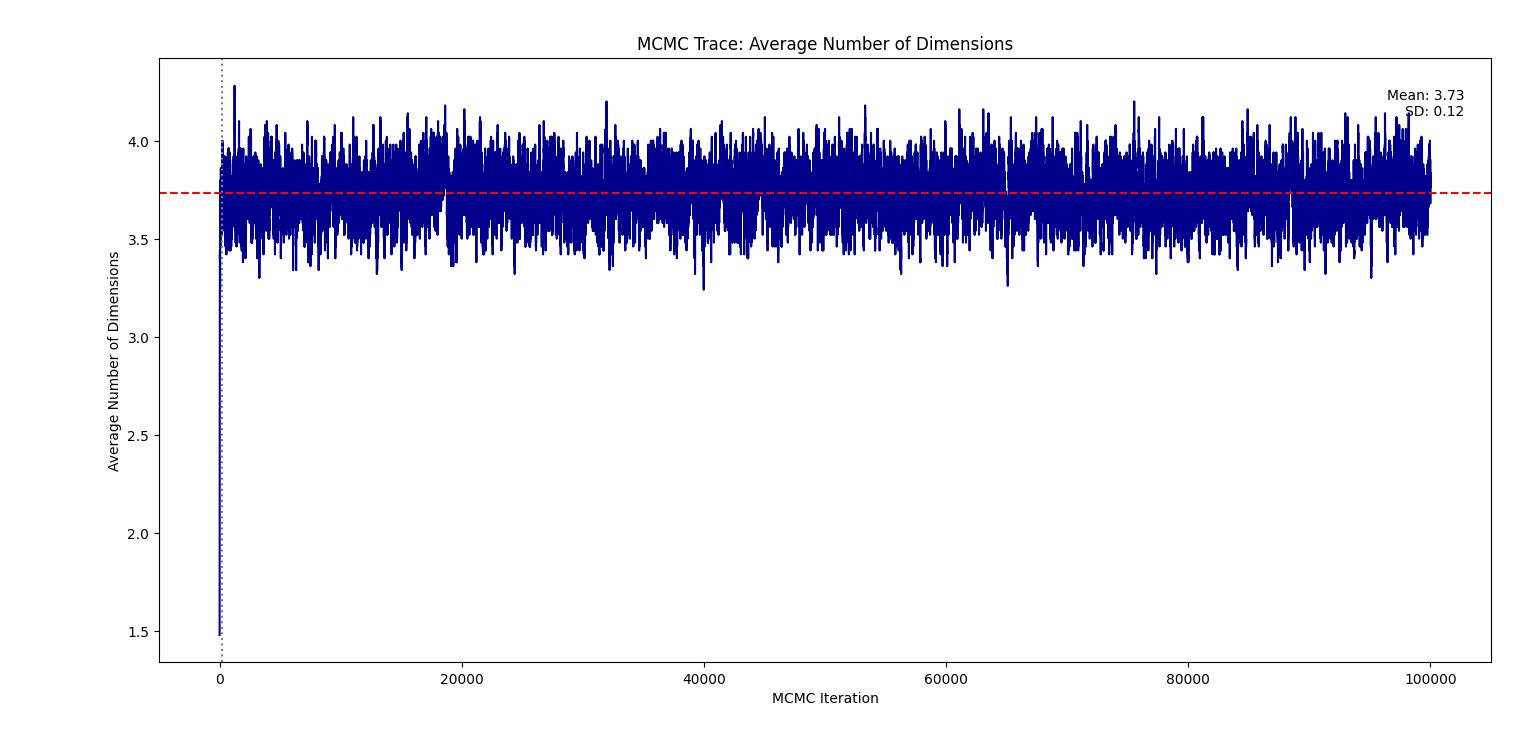
\includegraphics[width=0.8\textwidth]{plot1.png}
    \caption{Trace plot for average number of dimensions}
\end{figure}
\begin{figure}[H]
    \centering
    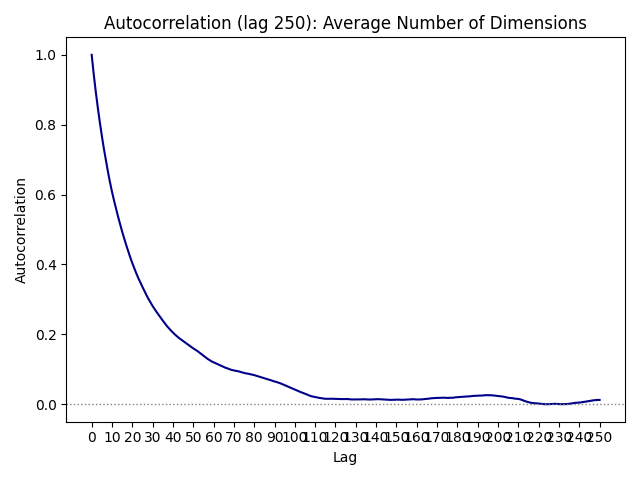
\includegraphics[width=0.8\textwidth]{plot3.png}
    \caption{Autocorrelation plot for average number of dimensions}
\end{figure}
\begin{figure}[H]
    \centering
    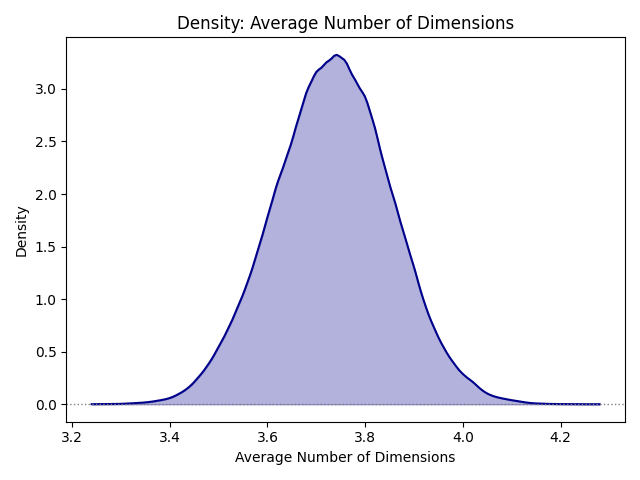
\includegraphics[width=0.8\textwidth]{plot2.png}
    \caption{Histogram for average number of dimensions}
\end{figure}
\newpage
\section{Earthquakes dataset}
In order to carry out further testing, we would need a well-produced large-scale dataset with a large number of covariates and observations. We were looking for something that used a variety of metrics, and had variables on varying scales. For that reason we decided to use the earthquakes dataset for further testing. The relevant files for this chapter can be found at \nolinkurl{benchmarks\ datasets\ earthquakes}\cite{repo}

\subsection{Data Source}

The raw data was obtained from the U.S. Geological Survey's Earthquake Hazards
Program, via the public ANSS Comprehensive Earthquake Catalog (ComCat) query API\cite{earthquakes-api}.

The pull used for this article consists of the most recent 20{,}000 earthquake
records in the catalog which occured in 2025 (magnitude $\geq 2.5$), which
corresponds to events occurring between 5 May 2025 and 31 December 2025. The USGS
API caps any single query at 20{,}000 returned rows; a full multi-decade pull
requires paginating over the \texttt{offset} parameter or splitting the request
into shorter date ranges, but the analysis in this article is restricted to this
single 20{,}000-row pull as a representative working sample.

The raw file, \texttt{raw\_data.csv}\cite{repo}, contained 20{,}000 rows and 19 columns:
\texttt{time}, \texttt{latitude}, \texttt{longitude}, \texttt{depth}, \texttt{mag},
\texttt{magType}, \texttt{nst}, \texttt{gap}, \texttt{dmin}, \texttt{rms},
\texttt{net}, \texttt{type}, \texttt{horizontalError}, \texttt{depthError},
\texttt{magError}, \texttt{magNst}, \texttt{status}, \texttt{locationSource}, and
\texttt{magSource}.

\subsection{Data Cleaning}

The raw data required six cleaning steps: (i) restricting to genuine earthquake
events, since the catalog also contains a small number of mining explosions and
other non-tectonic events; (ii) removing columns that were pure metadata,
near-duplicates of another retained column, or deliberately excluded from the
benchmark covariate set; (iii) removing the small proportion of rows with
residual missing values in the quality-control columns; (iv) subsetting to
reviewed body-wave magnitude events, i.e. \texttt{magType == "mb"} and
\texttt{status == "reviewed"}; and (v) dropping the now-constant
\texttt{magType}, \texttt{status}, and \texttt{net} columns from the retained covariate set.
The full cleaning pipeline, implemented in R, can be found at \nolinkurl{clean_earthquakes.R}\cite{repo}. Applying this pipeline reduced the raw extract from 20{,}000 rows and 19 columns
to a final cleaned dataset of 11{,}697 rows and 11 columns, with zero remaining
missing values. Table~\ref{tab:pipeline} summarises each stage.

\begin{table}[h]
\centering
\begin{tabular}{lrr}
\toprule
Stage & Rows & Columns \\
\midrule
Raw extract & 20{,}000 & 19 \\
After filtering to \texttt{type == "earthquake"} & 19{,}841 & 19 \\
After dropping redundant columns & 19{,}841 & 14 \\
After dropping incomplete rows & 18{,}732 & 14 \\
After subsetting to \texttt{magType == "mb"} and \texttt{status == "reviewed"} & 11{,}697 & 14 \\
After dropping constant \texttt{magType}, \texttt{status}, and \texttt{net} columns & 11{,}697 & 11 \\
\bottomrule
\end{tabular}
\caption{Row and column counts at each stage of the cleaning pipeline.}
\label{tab:pipeline}
\end{table}

\subsection{Covariate Descriptions}

Table~\ref{tab:covariates} describes each of the 11 covariates retained in the
final cleaned dataset, along with its type and the range (for numeric variables)
or levels (for categorical variables) observed in the data.

\begin{longtable}{p{2.6cm}p{1.6cm}p{6.3cm}p{3.5cm}}
\toprule
\textbf{Covariate} & \textbf{Type} & \textbf{Description} & \textbf{Range / Levels} \\
\midrule
\endfirsthead
\toprule
\textbf{Covariate} & \textbf{Type} & \textbf{Description} & \textbf{Range / Levels} \\
\midrule
\endhead

\texttt{latitude} & Numeric & Epicenter latitude in decimal degrees (WGS84). Natural great-circle covariate. & $-65.6^{\circ}$ to $87.1^{\circ}$ \\
\addlinespace
\texttt{longitude} & Numeric & Epicenter longitude in decimal degrees (WGS84). Natural great-circle covariate. & $-180.0^{\circ}$ to $180.0^{\circ}$ \\
\addlinespace
\texttt{depth} & Numeric & Depth of the hypocenter below the surface, in kilometers. Small negative values reflect very shallow events located slightly above the reference datum. & $-3.4$ to $669.6$ km \\
\addlinespace
\texttt{mag} & Numeric & Earthquake magnitude, on the body-wave scale used for the retained events. Natural target variable. & $2.5$ to $8.8$ \\
\addlinespace
\texttt{nst} & Numeric & Number of seismic stations used to determine the event's \emph{location}. & $3$ to $566$ \\
\addlinespace
\texttt{dmin} & Numeric & Horizontal distance, in degrees, from the epicenter to the nearest reporting station. & $0$ to $55.9$ \\
\addlinespace
\texttt{rms} & Numeric & Root-mean-square of the travel-time residuals, in seconds; a location goodness-of-fit measure. & $0$ to $2.0$ s \\
\addlinespace
\texttt{horizontalError} & Numeric & 95\% confidence radius on the epicenter location, in kilometers. & $0$ to $40.8$ km \\
\addlinespace
\texttt{depthError} & Numeric & 95\% confidence uncertainty on the depth estimate, in kilometers. & $0$ to $42.9$ km \\
\addlinespace
\texttt{magError} & Numeric & Standard error on the magnitude estimate, in magnitude units. & $0$ to $1.3$ \\
\addlinespace
\texttt{magNst} & Numeric & Number of seismic stations used to compute the \emph{magnitude} (distinct from \texttt{nst}). & $0$ to $1{,}027$ \\
\addlinespace
\bottomrule
\caption{Covariates in the cleaned earthquake dataset.}
\label{tab:covariates}
\end{longtable}
For the use of this dataset in testing, we used \texttt{mag}, the magnitude of the earthquake, as the response variable.
\section{Investigative testing using HPC resources}
For the sake of further testing, we made use of the Hamilton HPC service of Durham University. The code used to generate the following test results were written with the following properties in mind:
\begin{itemize}
\item Parallelism: With each compute node on Hamilton having 128 CPU cores, making effective use of parallel processing was crucial in speeding up tests
\item Pausable: For long processes which we would expect to take over a day to run, we designed test code such that a log of which point in the code execution was reached, so that if a process was interrupted, for example by a runtime error or system downtime, then the tests could be resumed from the same place.
\end{itemize}
The files referenced in this chapter can be found at \nolinkurl{AddiVortes\ testing}\cite{repo}
\subsection{Testing sensitivity of key metrics to parameter changes}
We wanted to better understand the impact of model parameter settings on two key metrics: model fit time, and out-of-sample RMSE. The important thing to try and observe here is whether there was a trade-off between these 2 values, and if so, at  which point do the improvements in out-of-sample RMSE start to diminish?\\\\
We first designed code to generate a factorial grid of possible model parameters. This simply gave parameters equally spaced values over their search range, being able to specify how many values were needed in each parameter range. This was our first, naive approach to the problem of hyperparameter optimisation, with the result being an equally spaced grid over parameter space. Whilst this doesn't consider how metrics may be affected by different parameters in different ways, it would give us a clearer idea of how changing certain parameters may affect metrics more than others.\\
\\
We considered the following parameters, which could be changed in the Python implementation: \texttt{m, nu, q, omega, lambda, iter, burnin} .The code used to generate the equally spaced factorial grid can be found at \nolinkurl{grid.py} and the output can be found at \nolinkurl{grid.csv}\cite{repo}.
\\
\begin{table}[h]
\begin{center}
\csvautotabular{grid_table.csv}
\caption{The first 10 rows of the factorial grid with 2 options for each parameter}
\end{center}
\end{table}
We then fit an AddiVortes model using each row of parameter settings from the grid, and recorded fit time, prediction time, and in-sample and out-of-sample RMSEs. The code used to run these tests is available at \nolinkurl{grid_tests.py} and the results are avaliable at \nolinkurl{grid-testlog.csv}
\\\\
TODO analysis of the partial results obtained. 
\subsection{Parameter screening}
In order to determine which parameters have a non-linear effect on the metrics, these being the parameters whose effect on the metrics would have to be investigated more closely, we carried out screening. The method used is built upon the elementary effects (EE) method for screening and uses a threshold value to separate the inputs with linear and nonlinear effects\cite{screening-paper}. The code used to implement this method can be found at \nolinkurl{AddiVortes\ screening}.\\\\ TODO screening analysis
\newpage
\bibliography{bibliography}
\end{document}
